\begin{titlepage}

\newcommand{\HRule}{\rule{\linewidth}{0.5mm}}
% \renewcommand{\baselinestretch}{2.0}
\centering
\begin{center}
\large ĐẠI HỌC QUỐC GIA THÀNH PHỐ HỒ CHÍ MINH \\
TRƯỜNG ĐẠI HỌC BÁCH KHOA \\
KHOA ĐIỆN - ĐIỆN TỬ  \\
BỘ MÔN VIỄN THÔNG  \\ [0.2cm]
\end{center}

\begin{figure}[!ht]
    \centering
    
\includegraphics[scale=0.3]{front_pages/Logo_BK.png}
    \label{fig:logo}
\end{figure}

%\centering
\bfseries
\Large{LUẬN VĂN TỐT NGHIỆP ĐẠI HỌC} \\[1.3cm]


\LARGE{NHẬN DẠNG NGÔN NGỮ KÝ HIỆU CHO  NGƯỜI KHIẾM THÍNH SỬ DỤNG KỸ THUẬT HỌC SÂU: TÁCH VÀ PHÂN TÍCH ĐẶC TRƯNG KHUNG XƯƠNG TRÊN VIDEO RGB} \\ [2.1cm]

\normalfont
\normalsize
% \small

\centering
\begin{tabular}{r l}
    \fontsize{14pt}{0pt}{\selectfont{GVHD:}} & \fontsize{14pt}{0pt}{\selectfont{PGS.TS HÀ HOÀNG KHA}} \\
    \fontsize{14pt}{0pt}{\selectfont{SVTH:}} & \fontsize{14pt}{0pt}{\selectfont{NGUYỄN THÀNH ĐẠT - 1510698}}  					
                        
\end{tabular} 
\\ [2.1cm]

\centering
TP. HỒ CHÍ MINH, THÁNG 12 NĂM 2019
% \vfill
\end{titlepage}


%------------------------------------------------------------------
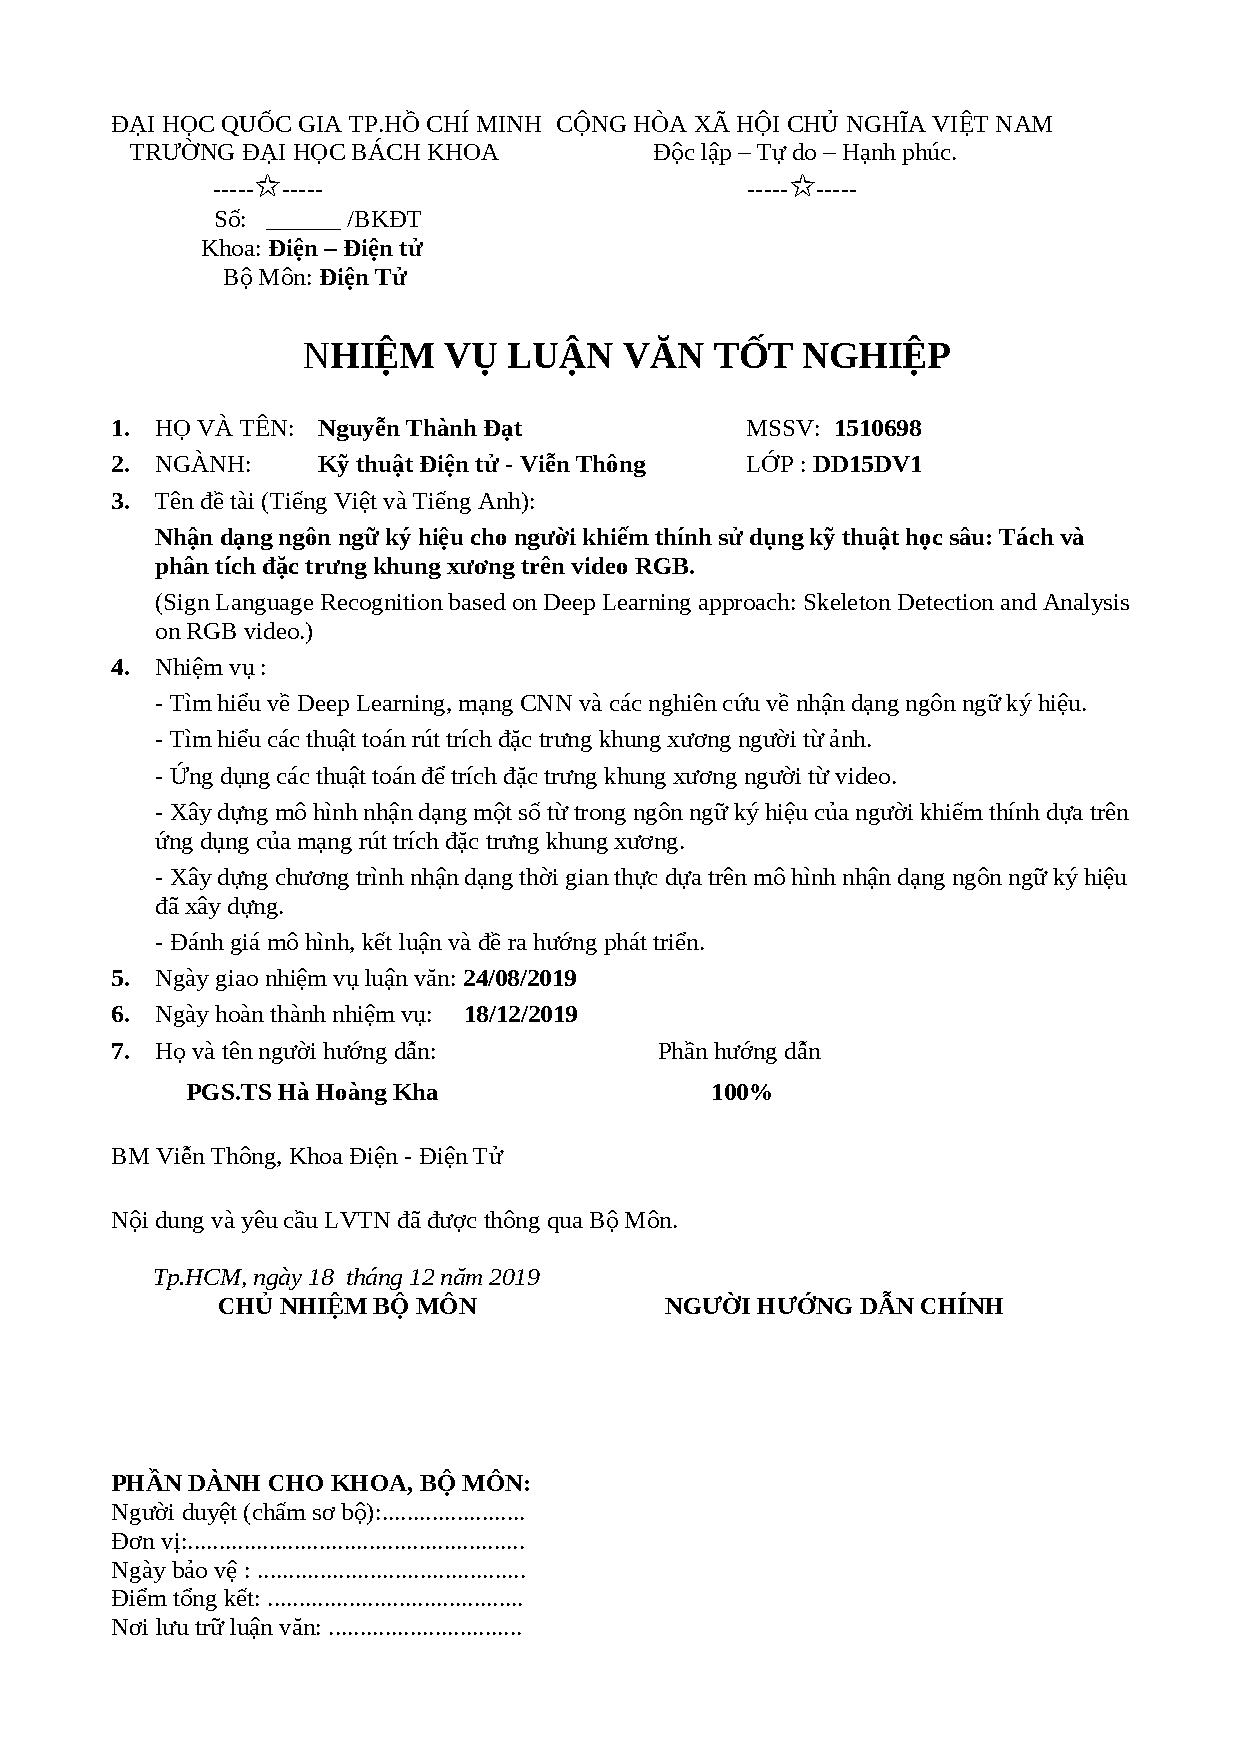
\includepdf[pages=-]{front_pages/nhiem_vu.pdf}

%------------------------------------------------------------------
\newpage
\pagenumbering{roman}
\addcontentsline{toc}{chapter}{LỜI CẢM ƠN}
\thispagestyle{loi_cam_on}
\begin{center}
{\fontsize{18pt}{30pt}{\selectfont{\textbf{Lời cảm ơn}}}}
\end{center}

\textit{Trong thời gian thực hiện luận án này, em đã nhận được sự hỗ trợ nhiệt tình, hướng dẫn tận tình và những lời động viên tích cực từ các giảng viên, bạn bè và gia đình. Nhờ những sự giúp đỡ đó, em đã hoàn thành được luận án như mục tiêu đã đặt ra. Những lời giảng dạy quý báu, không những về mặt kiến thức mà còn về đạo đức làm người của các quý thầy cô sẽ là hành trang cho con đường tương lai của các thế hệ sinh viên.}

\textit{Đặc biệt em xin gửi đến thầy Hà Hoàng Kha, giảng viên hướng dẫn trực tiếp đề tài, lời biết ơn sâu sắc. Thầy đã dành thời gian quý báu để gặp gỡ, thảo luận và rèn luyện chúng em khả năng giải quyết vấn đề. Thầy là người đã theo tường bước đi trong quá trình nghiên cứu luận văn, tận tình chỉ bảo, hướng dẫn chúng em từ khi làm đề cương, thực tập cho đến luận văn. Ngoài những kiến thức chuyên ngành, chúng em còn nhận được những lời khuyên, kinh nghiệm quý giá trong học tập và nghiên cứu từ thầy.}

\textit{Xin gửi lời cảm ơn đến "Giáo Dục Sáng Tạo" là tổ chức đã xây dựng nên bộ từ điển ngôn ngữ ký hiệu Việt Nam (\url{https://tudienngonngukyhieu.com/}). Từ điển đã là nguồn dữ liệu cũng như tư liệu tham khảo quý giá giúp quá trình nghiên cứu luận văn được thực hiện thuận lợi.}

\textit{Xin gửi lời cảm ơn đến các bạn bè đã dành công sức hỗ trợ mình từ việc thu thập dữ liệu đến động viên tinh thần cho mình trong những lúc khó khăn.}

\textit{Con cũng xin cảm ơn chân thành đến cha mẹ đã động viên và tạo điều kiện tốt nhất để em có thể chuyên tâm học tập và nghiên cứu luận văn.}

\textit{Cuối cùng, xin chân thành cảm ơn quý thầy cô và các bạn đã dành thời gian đọc luận văn này. Mặc dù đã cố gắng trong phạm vi và khả năng cho phép, nhưng luận văn không thể tránh khỏi những thiếu sót, rất mong được sự góp ý của quý thầy cô và các bạn.}


%\begin{flushright}

\begin{center}
\hspace{7cm} Tp.Hồ Chí Minh, ngày 18 tháng 12 năm 2019 \\
\hspace{7cm} Sinh viên \\
\hspace{7cm} Nguyễn Thành Đạt
\end{center}

%\end{flushright}


%------------------------------------------------------------------
\newpage
\addcontentsline{toc}{chapter}{LỜI CAM ĐOAN}
\thispagestyle{loi_cam_doan}
\begin{center}
{\fontsize{18pt}{30pt}{\selectfont{\textbf{Lời cam đoan}}}}
\end{center}

\noindent Tôi tên: Nguyễn Thành Đạt là sinh viên chuyên ngành Điện tử - Viễn thông khóa 2015 tại Đại học Quốc gia thành phố Hồ Chí Minh – Trường Đại học Bách Khoa. Tôi xin cam đoan Tôi xin cam đoan những nội dung sau đều là sự thật:
\begin{itemize}
\item Luận văn tốt nghiệp "Nhận dạng ngôn ngữ ký hiệu cho người khiếm thính sử dụng kỹ thuật học sâu: tách và phân tích đặc trưng khung xương trên video RGB" hoàn toàn do chính tôi thực hiện.
\item Các tài liệu và trích dẫn trong luận văn này được tham khảo từ các nguồn thực tế, có uy tín và độ chính xác cao.
\item Các số liệu và kết quả của công trình này được tôi tự thực hiện một cách độc lập và trung thực.
\end{itemize}

Nếu không thực hiện đúng các cam kết trên, tôi xin hoàn toàn chịu trách nhiệm trước kỷ luật của nhà trường cũng như pháp luật Nhà nước.
\\
[3cm]
\begin{center}
\hspace{7cm} Sinh viên thực hiện
\end{center}


%------------------------------------------------------------------
\newpage
\addcontentsline{toc}{chapter}{TÓM TẮT}
\thispagestyle{tom_tat}
\begin{center}
{\fontsize{18pt}{30pt}{\selectfont{\textbf{Tóm tắt}}}}
\end{center}

Trong luận văn này, em đã thực hiện viết ứng dụng realtime nhận diện được một số từ ngữ thông dụng trong ngôn ngữ ký hiệu của người khiếm thính Việt Nam trong giao tiếp. Ứng dụng được xây dựng với mục đích giúp cho người khiếm thính giao tiếp dễ dàng hơn với người bình thường khi họ không hiếu ngôn ngữ ký hiệu của người khiếm thính.

Bởi những phát triển trong học máy và học sâu gần đây, đã giúp con người giải quyết được những bài toán thực tế mà trước đây tưởng chừng như máy tính không thể làm được. Trong ứng dụng này em đã sử dụng một trong các phương pháp học máy đó để giải quyết bài toán nhận diện ngôn ngữ ký hiệu cho người khiếm thính Việt Nam. Phương pháp nhận diện mà đề tài sử dụng chia làm 2 bước chính. Đầu tiên từ hình ảnh RGB có chứa hình ảnh người khiếm thính đang diễn tả một từ ngữ do camera truyền vào. Ứng dụng sử dụng một mạng CNN dựa trên mạng mobilenet\_v2 để ước lượng tư thế con người (pose estimate). Mô hình sẽ dự đoán ra các vector đặc trưng khung xương (SJMs), là tọa độ các điểm khớp xương trên ảnh 2D (tổng cộng có 18 khớp xương ban đầu). Sau đó các vector đặc trưng này được xử lý đưa vào một mạng DNN để từ đó phân loại ra các hành động diễn tả từ ngữ mà mạng đã học được. Cuối cùng, ứng dụng xuất ra từ ngữ mà người đứng trước camera muốn diễn tả ra màn hình. Điểm quan trọng là mô hình này có thể xử lý đồng thời đối với nhiều người trong khung hình cùng một lúc. Ngoài ra ứng dụng còn sử dụng giải thuật Deep Sort để theo dõi từng người trong khung hình và các từ ngữ mà từng người diễn đạt. Ứng dụng tương tác với người sử dụng qua giao diện được viết bằng thư viện PyQt5. 

Phương pháp nhận diện dựa vào trích xuất đặc trưng khung xương là một phương pháp được sử dụng nhhiều trong nhận dạng hành động, nhận dạng dáng đi và nhiều bài toán khác. Điểm hay của phương pháp này là việc trích xuất khung xương đã khái quát gần như toàn bộ tư thế và hành động và tư thế mà con người diễn tả. Việc này còn làm giảm số chiều dữ liệu so với việc từ một hình ảnh RGB đưa vào để phân loại ra từ ngữ gì. Việc còn lại chỉ cần phân loại hành động dựa trên đặc trưng đã được trích xuất bằng một mạng DNN cấu trúc nhỏ. Việc này giúp tăng tốc độ xử lý của ứng dụng lên để đáp ứng được việc xử lý realtime. Các kết quả thực nghiệm thu được từ hệ thống cho thấy tỷ lệ nhận dạng cao và tốc độ đáp ứng đủ nhanh cho hoạt động chế độ thời gian thực.

%------------------------------------------------------------------
\newpage
\thispagestyle{abstract}
\begin{center}
{\fontsize{18pt}{30pt}{\selectfont{\textbf{ABSTRACT}}}}
\end{center}
%\textbf{Key words:} 
In this thesis, I have implemented realtime application to identify some common words in the sign language of Vietnamese deaf people in communication. The application was built with the purpose of helping the hearing impaired to communicate more easily with ordinary people when they are not fond of the sign language of the hearing impaired.

Because of recent developments in machine learning and deep learning, it has helped people solve real-world problems that previously seemed impossible to computers. In this application, I used one of the machine learning methods to solve the problem of sign language recognition for Vietnamese deaf people. The recognition method that the project uses is divided into 2 main steps. First from the RGB image contains the image of the hearing impaired expressing a word transmitted by the camera. The application uses a CNN network based on the mobilenet\_v2 network to estimate the pose of a person (pose estimate). The model predicts the "skeleton joints mapping" (SJMs), which are the coordinates of the joint points on the 2D image (a total of 18 initial joints). These feature vectors are then processed into a DNN network, which then categorizes the descriptive actions the network has learned. Finally, the application outputs the words that the person in front of the camera wants to describe to the screen. The important point is that this model can handle many people in the frame simultaneously. In addition, the application also uses the Deep Sort algorithm to track each person in the frame and the words that each person expresses. The application interacts with the user through the interface written in the PyQt5 library.

The identification method based on skeletal feature extraction is a method that is used a lot in action recognition, gait identification and many other problems. The beauty of this method is that the extraction of the skeleton has generalized almost the entire posture and action and posture that people describe. This also reduces the number of data dimensions compared to what an RGB image is inserted to sort out. The rest just needs to classify the action based on the feature extracted by a small structured DNN network. This increases the speed of the application to meet realtime processing. Experimental results obtained from the system show that the recognition rate is high and the response speed is fast enough for real-time mode operation.

%------------------------------------------------------------------
\newpage
\addcontentsline{toc}{chapter}{MỤC LỤC}
{\fontsize{12pt}{5pt}\selectfont
\tableofcontents}


%------------------------------------------------------------------
\newpage
\addcontentsline{toc}{chapter}{DANH SÁCH HÌNH VẼ}
\listoffigures


%------------------------------------------------------------------
\newpage
\addcontentsline{toc}{chapter}{DANH SÁCH BẢNG}
\listoftables


%------------------------------------------------------------------
\newpage
\thispagestyle{danhmucviettat}
\addcontentsline{toc}{chapter}{DANH MỤC TỪ VIẾT TẮT}
{\fontsize{18pt}{30pt}{\selectfont{\textbf{Danh mục từ viết tắt và các thuật ngữ tiếng anh}}}}


%CFMs & : Confidence Maps

\FloatBarrier
\begin{table}[h]
%\caption{Tổng quan các chương của luận văn}
\label{table:tu_viet_tat}
\centering
\begin{center}
\begin{tabular}{|c|l|p{7cm}|} 
\hline 
NN & Neural Network & Mạng thần kinh\\ 
\hline
CNN & Convolutional Neural Networks & Mạng neuron tích chập\\
\hline 
DNN & Deep Neural Network & Mạng thần kinh sâu\\
\hline
HMM & Hidden Markov Model & Mô hình Markov ẩn \\
\hline 
DL & Deep Learning & Học sâu\\
\hline
GD & Gradient Descent & Giảm theo gradient(tạm dịch)\\
\hline
SGD & Stochastic Gradient Descent & Giảm theo gradient ngẫu nhiên(tạm dịch)\\
\hline
RGB & red green blue & 3 kênh màu đỏ, xanh, vàng \\
\hline
SJM & Skeleton Joints Mapping & Vector đặc trưng mang hình dáng của khung xương con người\\
\hline
SJM-J & Skeleton Joints Mapping-Joint & Điểm khớp xương trong SJM\\
\hline
AF & Affinity Field &  Trường tương đồng (tạm dịch)\\
\hline
PAF & Part Affinity Field &  Trường tương đồng một phần (tạm dịch)\\
\hline
CFM & Confidence Map & Bản đồ tự tin(tạm dịch)\\
\hline
2D & 2-dimensional & 2 chiều \\
\hline
3D & 3-dimensional & 3 chiều \\
\hline
- & pose estimate & ước tính tư thế \\
\hline
- & bottom-up & từ dưới lên (tạm dịch) \\
\hline
- & realtime & thời gian thực \\
\hline
- & loss function & hàm lỗi, hàm mất mát \\
\hline
- & greedy algorithm & thuật toán tham lam \\
\hline
- & greedy inference & suy luận tham lam \\
\hline
\end{tabular}
\end{center}
\end{table}
\FloatBarrier
 
\newpage